% DO NOT COMPILE THIS FILE DIRECTLY!
% This is included by the other .tex files.

\begin{frame}[t,plain]
\titlepage
\end{frame}

\begin{frame}[t]{Contents of this presentation}
\begin{itemize}
	\item Progress
	\item Revised backlog
	\item Second sprint description 
	\item Final sprint 
	\item Feedback
\end{itemize}
\end{frame}


\begin{frame}[t]{Progress}

\framesubtitle{Starfish: a quick recap}

\begin{itemize}
  \item System to improve knowledge sharing
  \item Network of linked (directed) documents
  \item Goal: create system that can automaticaly propose new links
\end{itemize}


\end{frame}




\begin{frame}[t]{Progress}

  \huge{Sprint One or Week Two}

\end{frame}




\begin{frame}[t]{Progress}

\framesubtitle{What did we set out to do?}

% Hier moet een afbeelding van sprint 1 backlog in

\end{frame}

\begin{frame}[t]{Progress}

\framesubtitle{What did we do?}

\begin{itemize}
\item Software skeleton
\item Nearest Neighbor
\item Different vector distance metrics
\item Document vectorizers \\
  \begin{itemize}
    \item (Weighted) tag glossary descriptor
    \item Text descriptor
    \item Tag descriptor
    \item Smoothed tag descriptor
  \end{itemize}
\item Research on other methods
\end{itemize}

\end{frame}



\begin{frame}[t]{Progress}

\framesubtitle{What didn't we do?}

\begin{itemize}
\item Automated evaluation metric
\end{itemize}

\end{frame}



\begin{frame}[t]{Progress}

\framesubtitle{Deliverable}

A program that can given a network and a new document propose new
links between the new and known documents.

\addvspace{3mm}
{\tt \$ documentlinker\\ Usage: -vectorizer <algorithm> -distance <cosine/eucledian>}

\pause
\addvspace{3mm}
Does not accept a new document yet, but will propose new documents for every
document in the data set.

\end{frame}


\begin{frame}[t]{Product Backlog}
  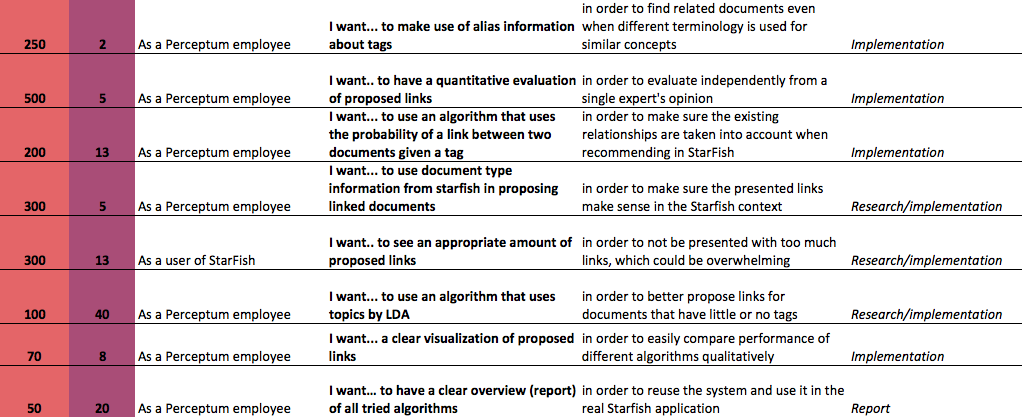
\includegraphics[width=\linewidth]{backlog2}
\end{frame}

\begin{frame}[t]{Definition of Done (recap)}
\framesubtitle{Product Backlog}

\begin{itemize}
	\item  The code is written OOP, and the classes that act correctly within the application framework
	\item The code is documented in a notebook containing examples of usage, test results and description of design choices 
	\item The code is well tested both individually as within the application flow (this may be done manually – no automated tests)
\end{itemize}
\end{frame}

\begin{frame}{Sprint 2}{Overview}
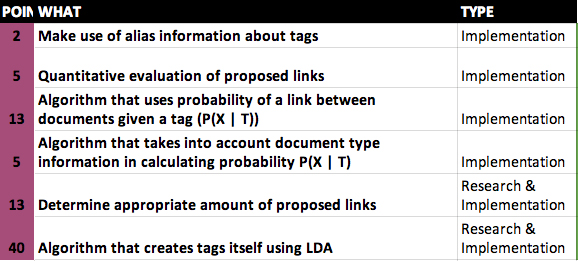
\includegraphics[width=\linewidth]{sprint.jpg}
\end{frame}

\begin{frame}{Sprint 2}{Replace aliased tags}
{\large 1. Make use of alias information about tags {\bf [2]}\\}
Each tag has a glossary, but some tags are aliases of each other and should use another tag's glossary. 
\end{frame}

\begin{frame}{Sprint 2}{Use links within the network }
{\large 'Semantic similarity' is different from heuristics used by StarFish experts.}\newline

{\large 2. Quantitative evaluation of proposed links {\bf [5]}\\}
{\bf Problem}: there are no proper links in current network\\
{\bf Solution}: network refined by expert, which will function as 'true network'
\center
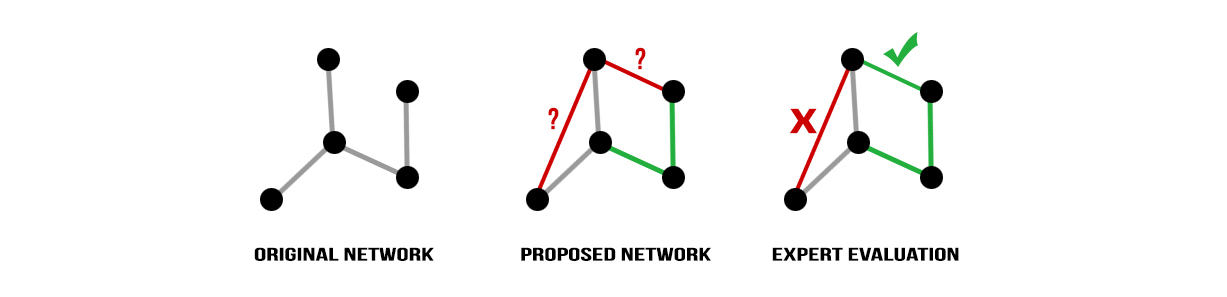
\includegraphics[width=\linewidth]{networks.jpg}
\end{frame}

\begin{frame}{Sprint 2}{Use links within the network }
{\large 3. Algorithm that uses probability of a link between documents given a tag (P(X | T)) {\bf [13]}}\\
Calculate $P(X | T) = \frac{P(T |X)P(X)}{P(T)}$, where X is an arbitrary link between two documents and T is a tag. \newline \newline
{\large 4. Algorithm that takes into account document type information in calculating probability P(X | T) {\bf[5]}}\\
Calculate $P(X | T)$ where X is a link from one particular type to another, e.g. $X = link(Person \rightarrow Question)$
\end{frame}

\begin{frame}{Sprint 2}{Usability}
{\large 5. Determine appropriate amount of proposed links{\bf [13]}}\\
Now the 10 best links are proposed, but sometimes less or more are really interesting.\newline \newline
{\bf Solution:} find proper threshold for Nearest Neighbor algorithm. 
\end{frame}

\begin{frame}{Sprint 2}{Dealing with missing tags}
{\large 6. Algorithm that creates tags itself using LDA {\bf[40]}}\\
{\bf Problem:} some documents have little or no tags\\
{\bf Solution:} generate 'tags' automatically using LDA, an algorithm that derivates topics from a data set.\newline \newline
Note: Difficult material, so not sure yet if we will manage to do this. 
\end{frame}

\begin{frame}{Sprint 3}{Short overview}
\begin{itemize}
\item Finish up all the code
\item Generating last results and analysis of those
\item Visualize last results
\item Writing of report
\end{itemize}

\end{frame}

\begin{frame}{Feedback}

{\large Thank you for listening!}\\
Are there any questions or suggestions?
\end{frame}

\begin{frame}[t]{Feedback}
We would love to hear what you think about our planning! Are there any suggestions or questions?
\end{frame}
